\section{Addition}
\label{sec:add}

Addition is the simplest of the basic arithmetic operators. It is a cornerstone
of arithmetics that can be used to define all other operations - an essential
part of a big integer library.

Former work has been carried out by students as part of a parallel course
project, which will serve as a stepping stone for the algorithm and
implementation of our addition \cite{DPPproject}.

This section is as follows: In subsection \ref{subsec:addalg} we present an
algorithm to compute big integer addition in parallel. In subsection
\ref{subsec:addcud} we discuss how to efficiently implement the algorithm on a
GPU in CUDA, and in subsection \ref{subsec:addfut} how to translate this
implementation to Futhark.

\subsection{Algorithm}
\label{subsec:addalg}

The additions of two big integers is the sum of the addition of their digits:
\begin{equation}
  \label{eq:add}
  u + v = \sum_{i=0}^{m-1}u_i\cdot B^{i} + \sum_{i=0}^{m-1}v_i\cdot B^{i} = \sum_{i=0}^{m-1}(u_i+v_i)\cdot B^{i}
\end{equation}

I.e. we can compute each digit of the result simply by adding the corresponding
two input digits. However, these additions may overflow the base size, which
results in a carry being added to the following digit. In turn, this digit may
now overflow, and so we need to add yet another carry, and so on. E.g. consider
the addition $199 + 1$ in decimal base; first we add $1$ to $9$ giving $0$ and a
carry, then we add $0$ and the carry to $9$ giving $0$ and another carry, which
we then add to $1$, resulting in the number $200$.

A sequential algorithm and illustration thereof is given in Figure
\ref{fig:addseq}. It is immidiate from the figure that the additions of digits
can be independently computed, and thus, trivially parallelizable. However, the
carries are dependent on all additions and carries before it.

\begin{figure}
  \centering
  \begin{minipage}{0.45\textwidth}
    \small
    \texttt{Input:} $u$ and $v$ of size $m$ base $B$\\
    \texttt{Output:} $w$ of size $m$ in base $B$
\begin{lstlisting}[language=pseudo,frame=]
c = 0
for i in (0..m-1)
    w[i] = u[i] + v[i] + c
    c = if overflow then 1 else 0
\end{lstlisting}
  \end{minipage}
  \begin{minipage}{0.45\textwidth}
    \centering
    \footnotesize
    \begin{tabular}{c}
      \begin{tabular}{|C{0.7cm}|C{0.7cm}|C{0.7cm}|C{0.7cm}|C{0.7cm}|}
        \hline
        $u_0$ & $u_1$ & $u_2$ & $\cdots$ & $u_{m-1}$\\ 
        \hline
      \end{tabular}\\
      \begin{tabular}{C{0.7cm}C{0.7cm}C{0.7cm}C{0.7cm}C{0.7cm}}
        $+$ & $+$ & $+$ & & $+$\\ 
      \end{tabular}\\
      \begin{tabular}{|C{0.7cm}|C{0.7cm}|C{0.7cm}|C{0.7cm}|C{0.7cm}|}
        \hline
        $v_0$ & $v_1$ & $v_2$ & $\cdots$ & $v_{m-1}$\\
        \hline
      \end{tabular}\\
      \begin{tabular}{C{0.7cm}C{0.7cm}C{0.7cm}C{0.7cm}C{0.7cm}}
        $+$ & $+$ & $+$ &  & $+$\\
      \end{tabular}\\
      \begin{tabular}{C{0.7cm}C{0.7cm}C{0.7cm}C{0.7cm}C{0.7cm}}
        $0$ & $c_1$ &  $c_2$ & $\cdots$ &$c_{m-1}$ \\
      \end{tabular}\\[-0.8ex]
      \begin{tabular}{C{0.15cm}C{0.15cm}C{0.15cm}C{0.15cm}C{0.15cm}C{0.15cm}C{0.15cm}}
       \diagonalarrow{} & & \diagonalarrow{} &  & \diagonalarrow{} &  & \diagonalarrow{}\\
      \end{tabular}\\[-2ex]
      \begin{tabular}{C{0.7cm}C{0.7cm}C{0.8cm}C{0.7cm}C{0.7cm}}
        $=$ & $=$ & $=$ &  & $=$  
      \end{tabular}\\
      \begin{tabular}{|C{0.7cm}|C{0.7cm}|C{0.7cm}|C{0.7cm}|C{0.7cm}|}
        \hline
        $w_{0}$ & $w_1$ & $w_2$ & $\cdots$ & $w_{m-1}$\\
        \hline
      \end{tabular}
    \end{tabular}
  \end{minipage}
  \caption{Pseudo-code and illustration of sequential addition algorithm.}
  \label{fig:addseq}
\end{figure}

Each addition may overflow at most once, and so we need to figure out when this
happens. In the former work by Olesen, Topalovic and Restelli-Nielsen, they
found that this happens when I) the addition already overflowed, or II) it
results in the maximum representable integer and the addition just before it
overflowed \cite{DPPproject}. This can be efficiently computed in parallel as a
prefix sum, specifically an exclusive one\footnote{Easy to see on the arrows of
  the illustration of the sequential algorithm in Figure \ref{fig:addseq}.}.

Thus, big integer addition parallelizes to a \fun{map}-\fun{scan} function
composition. Figure \ref{fig:addpar} lists and illustrates a generalized
parallel addition algorithm. The algorithm works in three steps: First, it
computes the result of the additions (\texttt{r}) and the augmented carries
(\texttt{a}) by mapping operator $\oplus$. Second, it computes a prefix sum
(\texttt{c}) over the augmented carries using operator $\otimes$ with left-associative
neutral element \texttt{e}. Third, it extracts the carries from the prefix sum
(using \texttt{f}) and adds them to the result of the additions over a map.

\begin{figure}
  \centering
  \begin{minipage}{0.47\textwidth}
    \footnotesize
    \texttt{Input:} $u$ and $v$ of size $m$ base $B$\\
    \texttt{Output:} $w$ of size $m$ in base $B$\\
    \texttt{Uses:} $f$ to extract carry from augmented carry
\begin{lstlisting}[language=pseudo,frame=,escapeinside={(*}{*)},name=paradd,backgroundcolor=\color{lightgray},]
(r, a) = map2 (*$\oplus$*) u v
\end{lstlisting}
\vspace{-\baselineskip}
\begin{lstlisting}[language=pseudo,frame=,escapeinside={(*}{*)},name=paradd,backgroundcolor=\color{Beige}]
c = scan_exc (*$\otimes$*) e a
\end{lstlisting}
\vspace{-\baselineskip}
\begin{lstlisting}[language=pseudo,frame=,escapeinside={(*}{*)},name=paradd,backgroundcolor=\color{LightSteelBlue}]
w = map2 ((*$\lambda$*) x y (*$\rightarrow$*) x + f y) r c
\end{lstlisting}
\end{minipage}
  \noindent\fcolorbox{white}{lightgray}{%
  \begin{minipage}{0.47\textwidth}
    \centering
    \footnotesize
    \begin{tabular}{c}
      \begin{tabular}{|C{0.7cm}|C{0.7cm}|C{0.7cm}|C{0.7cm}|C{0.7cm}|}
        \hline
        $u_0$ & $u_1$ & $u_2$ & $\cdots$ & $u_{m-1}$\\ 
        \hline
      \end{tabular}\\
      \begin{tabular}{C{0.7cm}C{0.7cm}C{0.7cm}C{0.7cm}C{0.7cm}}
        $\oplus$ & $\oplus$ & $\oplus$ & & $\oplus$\\ 
      \end{tabular}\\
      \begin{tabular}{|C{0.7cm}|C{0.7cm}|C{0.7cm}|C{0.7cm}|C{0.7cm}|}
        \hline
        $v_0$ & $v_1$ & $v_2$ & $\cdots$ & $v_{m-1}$\\
        \hline
      \end{tabular}\\
      \begin{tabular}{C{0.7cm}C{0.7cm}C{0.8cm}C{0.7cm}C{0.7cm}}
        $=$ & $=$ & $=$ &  & $=$  
      \end{tabular}\\
      \begin{tabular}{|C{0.7cm}|C{0.7cm}|C{0.7cm}|C{0.7cm}|C{0.7cm}|}
        \hline
        $r_{0}$ & $r_1$ & $r_2$ & $\cdots$ & $r_{m-1}$\\
        \hline
      \end{tabular}\\
      \begin{tabular}{C{0.15cm}C{0.15cm}C{0.15cm}C{0.15cm}C{0.15cm}C{0.15cm}C{0.15cm}}
        & &  &  &  &  & \\
      \end{tabular}\\[-2ex]
      \begin{tabular}{|C{0.7cm}|C{0.7cm}|C{0.7cm}|C{0.7cm}|C{0.7cm}|}
        \hline
        $a_{0}$ & $a_1$ & $a_2$ & $\cdots$ & $a_{m-1}$\\
        \hline
      \end{tabular}\\
    \end{tabular}
  \end{minipage}
  }\\
  \noindent\fcolorbox{white}{Beige}{%
    \begin{minipage}{0.4525\textwidth}
    \centering
    \scriptsize
    \begin{tabular}{c}
      \begin{tabular}{|C{0.7cm}|C{0.7cm}|C{0.7cm}|C{0.7cm}|C{0.7cm}|}
        \hline
        $a_{0}$ & $a_1$ & $a_2$ & $\cdots$ & $a_{m-1}$\\
        \hline
      \end{tabular}\\
      \begin{tabular}{C{0.15cm}C{0.15cm}C{0.15cm}C{0.15cm}C{0.15cm}C{0.15cm}C{0.15cm}C{0.15cm}C{0.15cm}C{0.15cm}C{0.15cm}}
        \texttt{e}$\shortrightarrow$ & $\otimes$ & $\shortrightarrow$ & $\otimes$ & $\shortrightarrow$ & $\otimes$ & $\shortrightarrow$ & $\otimes$ & $\shortrightarrow$ & $\otimes$ & \\
      \end{tabular}\\[-1.2ex]
      \begin{tabular}{C{0.15cm}C{0.15cm}C{0.15cm}C{0.15cm}C{0.15cm}C{0.15cm}C{0.15cm}C{0.15cm}C{0.15cm}C{0.15cm}C{0.15cm}}
       \diagonalarrowdown{} & & \diagonalarrowdown{} & & \diagonalarrowdown{} &  & \diagonalarrowdown{} &  & \diagonalarrowdown{} & &\\
      \end{tabular}\\[-0.3ex]
      \begin{tabular}{|C{0.7cm}|C{0.7cm}|C{0.7cm}|C{0.7cm}|C{0.7cm}|}
        \hline
        $c_{0}$ & $c_1$ & $c_2$ & $\cdots$ & $c_{m-1}$\\
        \hline
      \end{tabular}
    \end{tabular}
  \end{minipage}
}
\noindent\fcolorbox{white}{LightSteelBlue}{%
  \begin{minipage}{0.47\textwidth}
    \centering
    \footnotesize
    \begin{tabular}{c}
      \begin{tabular}{|C{0.7cm}|C{0.7cm}|C{0.7cm}|C{0.7cm}|C{0.7cm}|}
        \hline
        $r_0$ & $r_1$ & $r_2$ & $\cdots$ & $r_{m-1}$\\ 
        \hline
      \end{tabular}\\
      \begin{tabular}{C{0.7cm}C{0.7cm}C{0.7cm}C{0.7cm}C{0.7cm}}
        $\lambda$ & $\lambda$ & $\lambda$ & & $\lambda$\\ 
      \end{tabular}\\
      \begin{tabular}{|C{0.7cm}|C{0.7cm}|C{0.7cm}|C{0.7cm}|C{0.7cm}|}
        \hline
        $c_0$ & $c_1$ & $c_2$ & $\cdots$ & $c_{m-1}$\\
        \hline
      \end{tabular}\\
      \begin{tabular}{C{0.7cm}C{0.7cm}C{0.8cm}C{0.7cm}C{0.7cm}}
        $=$ & $=$ & $=$ &  & $=$  
      \end{tabular}\\
      \begin{tabular}{|C{0.7cm}|C{0.7cm}|C{0.7cm}|C{0.7cm}|C{0.7cm}|}
        \hline
        $w_{0}$ & $w_1$ & $w_2$ & $\cdots$ & $w_{m-1}$\\
        \hline
      \end{tabular}\\
    \end{tabular}
  \end{minipage}
  }
  \caption{Pseudo-code and illustration of parallel addition algorithm.}
  \label{fig:addpar}
\end{figure}

The task at hand is to figure out what $\oplus$, $\otimes$ and \texttt{e} is. In the former
work, Olesen et al. found $\oplus$ to compute whether the addition overflows or is
the maximum representable integer as a pair of boolean values s.t. for digits
$x$ and $y$ represented as unsigned integers in base $B$ with wrapping on
overflow, we define:
\begin{equation}
\label{eq:oplus}
x \oplus y \coloneq \tup{x + y < x}{x + y = B-1}
\end{equation}

The operator $\otimes$ then computes the prefix sum on the augmented carries s.t. if
both the addition itself and the one just before it results in the maximum
integer, then they remain the maximum integer combined, and overflows are
determined by the aforementioned conditions. For some pairs of booleans
$x = \tup{\mathit{ov_x}}{\mathit{mx_{x}}}$ and
$y = \tup{\mathit{ov_y}}{\mathit{mx_{y}}}$, we define:
\begin{equation}
  \label{eq:otimes}
  x \otimes y \coloneq \tup{\mathit{ov_x} \land \mathit{mx_y} \lor \mathit{ov_y}}{\mathit{mx_x} \land \mathit{mx_y}}
\end{equation}

They found that the neutral element, \texttt{e}, of $\otimes$ is:
\begin{equation}
  \label{eq:otimesne}
  \mathtt{e} \coloneq \tup{\mathtt{False}}{\mathtt{True}}
\end{equation}

While this approach is intuitive and straightforward to implement, hardware does
not support boolean values natively - they are syntactic sugar for
zero-and-nonzero integer words. Thus, a low-level implementation will have to
use integers, and so we might as well use bitwise operations over logical ones, as
these are faster.

In turn, instead of using pairs of integer words with only one indicator bit for
boolean values each, we combine them to one word with two bits used to each
indicate both boolean value. Not only does this halve the memory usage
w.r.t. the prefix sum, it also increases memory utilization as each workthread
only having to fetch and write one word.

The formalization of these optimizations, where the least and second least
significant bit indicates integer overflow and maximum representable integer,
respectively, is:
\begin{align}
  \label{eq:oplusopt}
  x \oplus y &\coloneq (x + y < x)~|~((x + y = B-1) \ll 1) \\
  \label{eq:otimesopt}
  x \otimes y &\coloneq (((x~\&~(y \gg 1))~|~y)~\&~1)~|~(x~\&~y~\&~2)\\
  \label{eq:otimesneopt}
  \mathtt{e} &\coloneq 2
\end{align}

Equation (\ref{eq:oplusopt}) is a straightforward conversion of equation
(\ref{eq:oplus}), with the pair being replaced by the shift- and bitwise or-operator.

Equation (\ref{eq:otimesopt}) is a conversion of equation (\ref{eq:otimes}),
where I) the pair is replaced with bitwise or-operator, II) the first clause is checked
in the least significant bit and zeroes out the second bit with ``$\&~1$'', and
III) the second clause is checked in the second least significant bit and zeroes
out the first bit with ``$\&~2$''. Associtivity naturally still holds:

\begin{proof}
  We want to show $x \otimes (y \otimes z) = (x \otimes y) \otimes z$. From left-to-right we have:
\begin{align}
  (x \otimes y) \otimes z &= (~\underbrace{(((x~\&~(y \gg 1))~|~y)~\&~1)~|~(x~\&~y~\&~2)}_{\alpha}~) \otimes z\\
              &= (((\alpha~\&~(z \gg 1))~|~z)~\&~1)~|~(\alpha~\&~z~\&~2)\\
              \label{eq:otimesproofltr}
              &= (((\alpha~\&~1)~\&~(z \gg 1))~|~(z~\&~1))~|~((\alpha~\&~2)~\&~z)
\end{align}
From right-to-left we have:
\begin{align}
  x \otimes (y \otimes z) &= x \otimes (~\underbrace{((y~\&~(z \gg 1))~|~z)~\&~1)~|~(y~\&~z~\&~2)}_{\beta}~)\\
  &= (((x~\&~(\beta \gg 1))~|~\beta)~\&~1)~|~(x~\&~\beta~\&~2)\\
  \label{eq:otimesproofrtl}
  &= ((x~\&~(\beta \gg 1)~\&~1)~|~(\beta~\&~1))~|~(x~\&~(\beta~\&~2))
\end{align}
We must now show that equation (\ref{eq:otimesproofltr}) is equal to
(\ref{eq:otimesproofrtl}). Consider the second clause. Since $(1~\&~2)$ is $0$,
so is the first clause of both $(\alpha~\&~2)$ and $(\beta~\&~2)$. Futhermore, we have
that $2~\&~2$ is the same as $2$. Thus, we have:
\begin{align}
  (\alpha~\&~2)~\&~z &= (x~\&~y~\&~2)~\&~z\\
                &= x~\&~(y~\&~z~\&~2)\\
                &= x~\&~(\beta~\&~2)
\end{align}
Consider the first clause. Again, $(2~\&~1)$ is $0$, so the second clause of $(\alpha~\&~1)$ is $0$:
\begin{align}
  ((\alpha~\&~1)~\&~&(z \gg 1))~|~(z~\&~1) \\
               &= ((((x~\&~(y \gg 1))~|~y)~\&~1)~\&~(z \gg 1))~|~(z~\&~1) \\
               &= (((x~\&~(y \gg 1)~\&~1)~|~(y~\&~1))~\&~(z \gg 1))~|~(z~\&~1) \\
               &= ((x~\&~(y \gg 1)~\&~(z \gg 1)~\&~1)~|~(y~\&~(z \gg 1)~\&~1))~|~(z~\&~1)
\end{align}
We have $((y \gg 1)~\&~(z \gg 1)) = (y~\&~z \gg 1) = (y~\&~z~\&~2 \gg 1)$ and get:
\begin{align}
  &= (x~\&~((y~\&~z~\&~2) \gg 1)~\&~1)~|~(y~\&~(z \gg 1)~\&~1)~|~(z~\&~1))\\
  \phantom{((\alpha~\&~1)\&}&= (x~\&~((y~\&~z~\&~2) \gg 1)~\&~1)~|~((y~\&~(z \gg 1))~|~z)~\&~1)\\
  &= (x~\&~(\beta \gg 1)~\&~1)~|~(\beta~\&~1)
\end{align}
Thus, equations (\ref{eq:otimesproofltr}) and (\ref{eq:otimesproofrtl}) are equal, and hence, $x \otimes (y \otimes z) = (x \otimes y) \otimes z$.
\end{proof}

Likewise, the netrual element \texttt{e} of Equation (\ref{eq:otimesneopt}) is
the corresponding indicator bits of Equation (\ref{eq:otimesne}), and so
\texttt{e} remains a left-associative neutral element of $\otimes$ after the
optimizations:

\begin{proof} By exhaustive evaluation we have:
\begin{align}
  \label{eq:otimesneproof}
  2 \otimes 0 &= (((2~\&~(0 \gg 1))~|~0)~\&~1)~|~(2~\&~0~\&~2) = 0 \\
  2 \otimes 1 &= (((2~\&~(1 \gg 1))~|~1)~\&~1)~|~(2~\&~1~\&~2) = 1 \\
  2 \otimes 2 &= (((2~\&~(2 \gg 1))~|~2)~\&~1)~|~(2~\&~2~\&~2) = 2 \\
  2 \otimes 3 &= (((2~\&~(3 \gg 1))~|~3)~\&~1)~|~(2~\&~3~\&~2) = 3
\end{align}
\end{proof}

Thus, when using the parallel algorithm presented in Figure \ref{fig:addpar}
with $\oplus$, $\otimes$ and \texttt{e} defined in Equations (\ref{eq:oplus}),
(\ref{eq:otimesne}) and (\ref{eq:otimesneopt}), we get that
$\mathtt{f} \coloneq 1~\&$. Both $\oplus$, $\otimes$ and \texttt{f} are $O(1)$, and so the
\fun{map}s exhibit work $O(m)$ and span $O(1)$, and the \fun{scan} work $O(m)$
and span $O(\log m)$. Thus, the work of a parallel big integer addition is
$O(m)$ and the span is $O(\log m)$.


\subsection{CUDA Implementation}
\label{subsec:addcud}

In this section we introduce three versions of addition in CUDA. The first
version (\texttt{V1}) is the fundamental implementation that follows the
algorithm presented in Figure \ref{fig:addpar} closely. The second version
(\texttt{V2}) attempts to efficiently sequentialize the parallelism in excess:
Since the operation runs in sublinear time, with two of the three steps being a
constant time, we expect the threads to have an excess amount of parallelism
spent on communication (waiting for memory and syncronizations). Upping the
sequentialization factor decreases the amount of communication, which may up the
performance. This version also serves to compute addition for integers of
greater size than a CUDA block. The third version (\texttt{V3}) conjoins
integers and do a segmented addition, giving better performance for multiple
arithmetic instances with small integer sizes, as mentioned in section
\ref{sec:strat}.

We determine the sequentialization factor ($q$), number of instances per block
($\mathit{ipb}$), and kernel dimensions with the code of Listing \ref{addparams}
below. Here, $v$ determines the version we want to run and
$\mathit{num\_instances}$ the total number of instances to add. Here we use a
trick; $(a + b - 1) / b = \lceil a / b \rceil$. The sequentialization factor
$q=4$ is determined experimentally to be the most efficient, and likewise for
$\mathit{ipb} = \lceil 256 / (m/q) \rceil$, which rounds the number of threads per block
up to 256.
\begin{lstlisting}[language=CPP,caption={CUDA addition parameters and kernel dimensions.},label={addparams}]
const uint32_t q = (v == 1) ? 1 : (m <= 1024) ? 4 : (m+1024-1) / 1024;
const uint32_t ipb = (v == 3) ? (256 + m/q - 1) / (m/q) : 1;
dim3 block(ipb*(m/q), 1, 1);
dim3 grid (num_instances/ipb, 1, 1);
\end{lstlisting}

Step 1. and step 3. are implemented straightforward for all three versions, by
simply computing the mapped functions. Step 2. on the other hand is a bit more
interresting.

For the \fun{scan} function, we have used the warp-level inclusive scan
presented in course \textit{Programming Massively Parallel Hardware}
\cite{PMPH}. The idea is to minimize communication by exploiting warps, since
warps execute instructions in lockstep. Figure \ref{fig:warpscan} contains an
illustration of this algorithm. It works in three steps; I) scan each warp, II)
scan the results at the end of warps, and III) distribute the results of "II)"
over the results "I)".

\begin{figure}
  \centering
  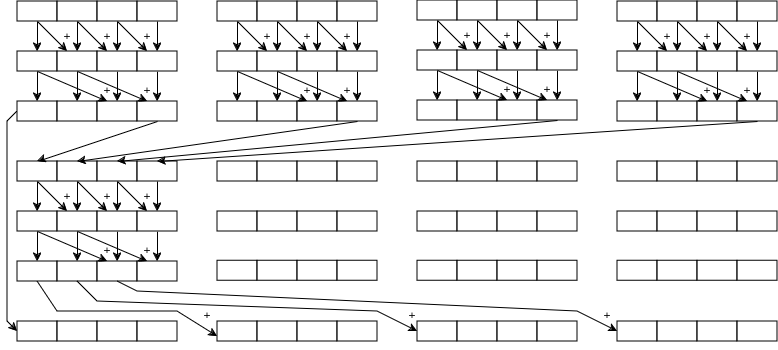
\includegraphics[width=0.8\textwidth]{img/warp-level-scan.png}
  \caption{Illustration of a warp-level inclusive scan with warp-size 4 and 16 threads}
  \label{fig:warpscan}
\end{figure}

To convert an inclusive to an exclusive scan, we shift the result to the right
by $1$ and insert the neutral element at the left-most position. Step 2. uses a
warp-level exclusive scan with the scan operator $\otimes$ and neutral element
$\mathtt{e}$ defined straightforward as Equations (\ref{eq:otimesopt})
(\ref{eq:otimesneopt}).

What we have so far is enough to write \texttt{V1}, but \texttt{V2} and
\texttt{V3} requires some extra steps. For \texttt{V2}, we have $q$ elements per
thread, and so we cannot directly use the defined scan (as this works for one
element per thread). Instead, let us reuse the "scan $\shortrightarrow$
end-of-result $\shortrightarrow$ scan $\shortrightarrow$ distribute" idea from
the scan algorithm:

Let each thread compute the inclusive prefix sum of its $q$ elements. Then,
compute a wrap-level exclusive scan over the
end-of-thread-level-scan-results. Lastly, distribute the results of the
wrap-level scan over the results of the thread-level scan.

In the kernel code, where the $q$ elements handled on a thread-level is in
$\mathtt{ass}$ and $\mathtt{bss}$ and output in $\mathtt{rss}$, shared memory
buffer $\mathtt{shmem}$, base $\mathtt{Base}$ and $\otimes$ as class
$\mathtt{CarryProp}$, we have:

\lstinputlisting[language=CPP,firstline=126,lastline=144,caption={\footnotesize CUDA addition with parameterized sequentialization (version 2) from file \texttt{ker-add.cu.h}.},label={addopcuda},firstnumber=126]{../cuda/ker-add.cu.h}

Lastly, $\mathtt{V3}$ is implemented in the same manner as $\mathtt{V2}$, but
segmented. A segmented scan is a scan with a flag array (indicating where new
segments starts) s.t. if we are at the begining of a segment, the neutral
element is used as the second operand rather than the left sum.

We can implement it as a normal scan, but with an extended operator that checks
segment beginings. Just like we combined the overflow-indicator and
maximum-integer-indicator, we can also combine them with the
segment-start-indicator (flag array). Thus, in the implementation, we use the
third least-significant bit to indicate segment beginings, and we get the
segmented scan operator $\otimes$ (still with neutral element $2$):
\begin{align}
  \label{eq:segscanop}
  x \otimes y &\coloneq x_f~|~y_f~|~\begin{cases} y_v & \textbf{if}~y_f \neq 0 \\ (((x_v~\&~(y_v \gg 1))~|~y_v)~\&~1)~|~(x_v~\&~y_v~\&~2) & \textbf{otherwise}\end{cases}\\
  & \textbf{where}~~x_f\coloneq (x~\&~4),~~x_v\coloneq (x~\&~3),~~y_f\coloneq (y~\&~4),~~y_v\coloneq (y~\&~3)\notag
\end{align}

Computing the flags before the scan and extracting the carries after the scan,
are trivial computations added to the \texttt{map}s of steps 1. and 3. of the
parallel addition algorithm.

\subsection{Futhark Implementation}
\label{subsec:addfut}

%%% Local Variables:
%%% mode: LaTeX
%%% TeX-master: "../main"
%%% End:
